%% -*- coding:utf-8 -*-

\settowidth\jamwidth{(German)}


\chapter{Phenomena}

This chapter deals with variation in the Germanic languages in what is often called the Core
Grammar, that is in sentences of the \emph{John loves Mary} variety.\footnote{%
  \citet[\page 7--8]{Chomsky81a} suggests dividing grammars of natural languages into a ``core'' part and a ``periphery''.
All regular parts belong to the core. The core grammar of a language is assumed to be an instance of
Universal Grammar (UG), the genetically determined innate language faculty of human beings. Idioms
and other irregular parts of a language belong to the periphery. This book deals with phenomena
usually assumed to be the core without assuming this core/periphery distinction and without assuming
a UG \citep{MuellerKernigkeit,MuellerCoreGram}.
} We will look at differences in
the verb position (verb before object and object before verb), the verb"=second property, which
all of the Germanic languages with the exception of English have, the ordering of subjects and
objects with respect to each other, the placement of adverbials, the existence/non-existence of
verbal complexes, the obligatoriness/absence of subjects, passive including the personal and
impersonal passive, expletive pronouns and various ways to mark the \isi{clause type}, that is, to
signal whether a certain clause is an assertion, a question or an embedded clause.

The purpose of this chapter is to set the scene for the chapters to come. It provides a general
discussion of the phenomena covered in this book. This will be repeated and extended in Chapter~\ref{chap-valence}--\ref{chap-expletives}.

A note of caution is necessary here: especially the following three subsections are potentially
confusing. A language like German will be categorized as an subject-object-verb language, a verb-second language and
a language with free constituent order \citep{Haftka96a}. This sounds contradictory but it is not. The respective
classifications refer to properties of languages as such, not to the form of single sentences.

\section{Order of subject, object and verb}
\label{sec-intro-svo}

The languages of the world can be classified according to the order of subject, object, and verb
that is dominant \citep{Greenberg63a-u}. In order to make languages comparable a very general definition of grammatical
functions like subject and object is used
for such a classification. The definition is based on semantic properties: subjects are those
arguments that are agent-like and objects are arguments that are rather patient like. This definition
is not always identical to the language-particular definitions. For instance, if one follows the
semantic definition, the phrase \emph{der
  Aufsatz} `the paper' in (\mex{1}) is the subject although it is inanimate and not an agent: 
\ea
\gll Der Aufsatz interessiert mich.\\
     the paper   interests    me\\
\glt `I am interested in the paper.'
\z
The language-particular definition of subject in German (and the Germanic languages in general)
rather refers to properties like nominative case, subject-verb-agreement, and control. We will deal with this in more
detail in Section~\ref{sec-subj-properties}.

Figure~\vref{fig-sov-wals} shows the dominant order of subject, object, and verb among the world's languages.
According to \citet{Dryer2013a} the dominant order is defined as follows:

%Dominante Abfolge (Dryer: Determining Dominant Word Order):
\begin{quote}
Where a language is shown on one of the word order maps as having a particular order as the dominant
order in the language, this means that it is either the only order possible or the order
that is more frequently used. \citep{Dryer2013a}
\end{quote}
%
%% I base my classification of Macushi here on the frequency counts, and since no order is more than
%% twice as frequent as the next most frequent order, I treat this language as lacking a dominant order
%% of subject, object, and verb.
%
%% Deutsch, Niederländisch und Friesisch sind V2-Sprachen, that is die SVO- und SVAuxOV-Stellungen kommen
%% durch die Voranstellung des Verbs zustande, die eine Funktion hat. Wir zählen diese Sprachen also
%% mit zu den SOV-Sprachen.
%
\begin{figure}
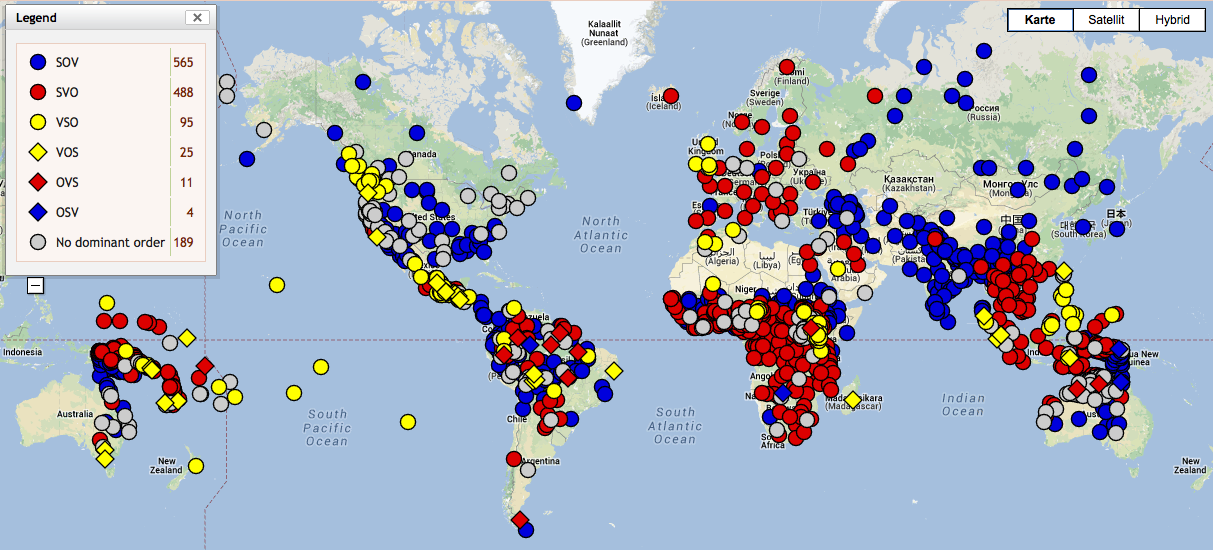
\includegraphics[width=\textwidth]{Pictures/WALS-SOV}
\caption{\label{fig-sov-wals}\citet[Section~1]{Dryer2013c}: Feature 81A: Order of subject, object and verb, The World Atlas of Language Structures} 
\end{figure}

If we zoom in to display the European languages we get Figure~\vref{fig-sov-wals-europe}.
\begin{figure}
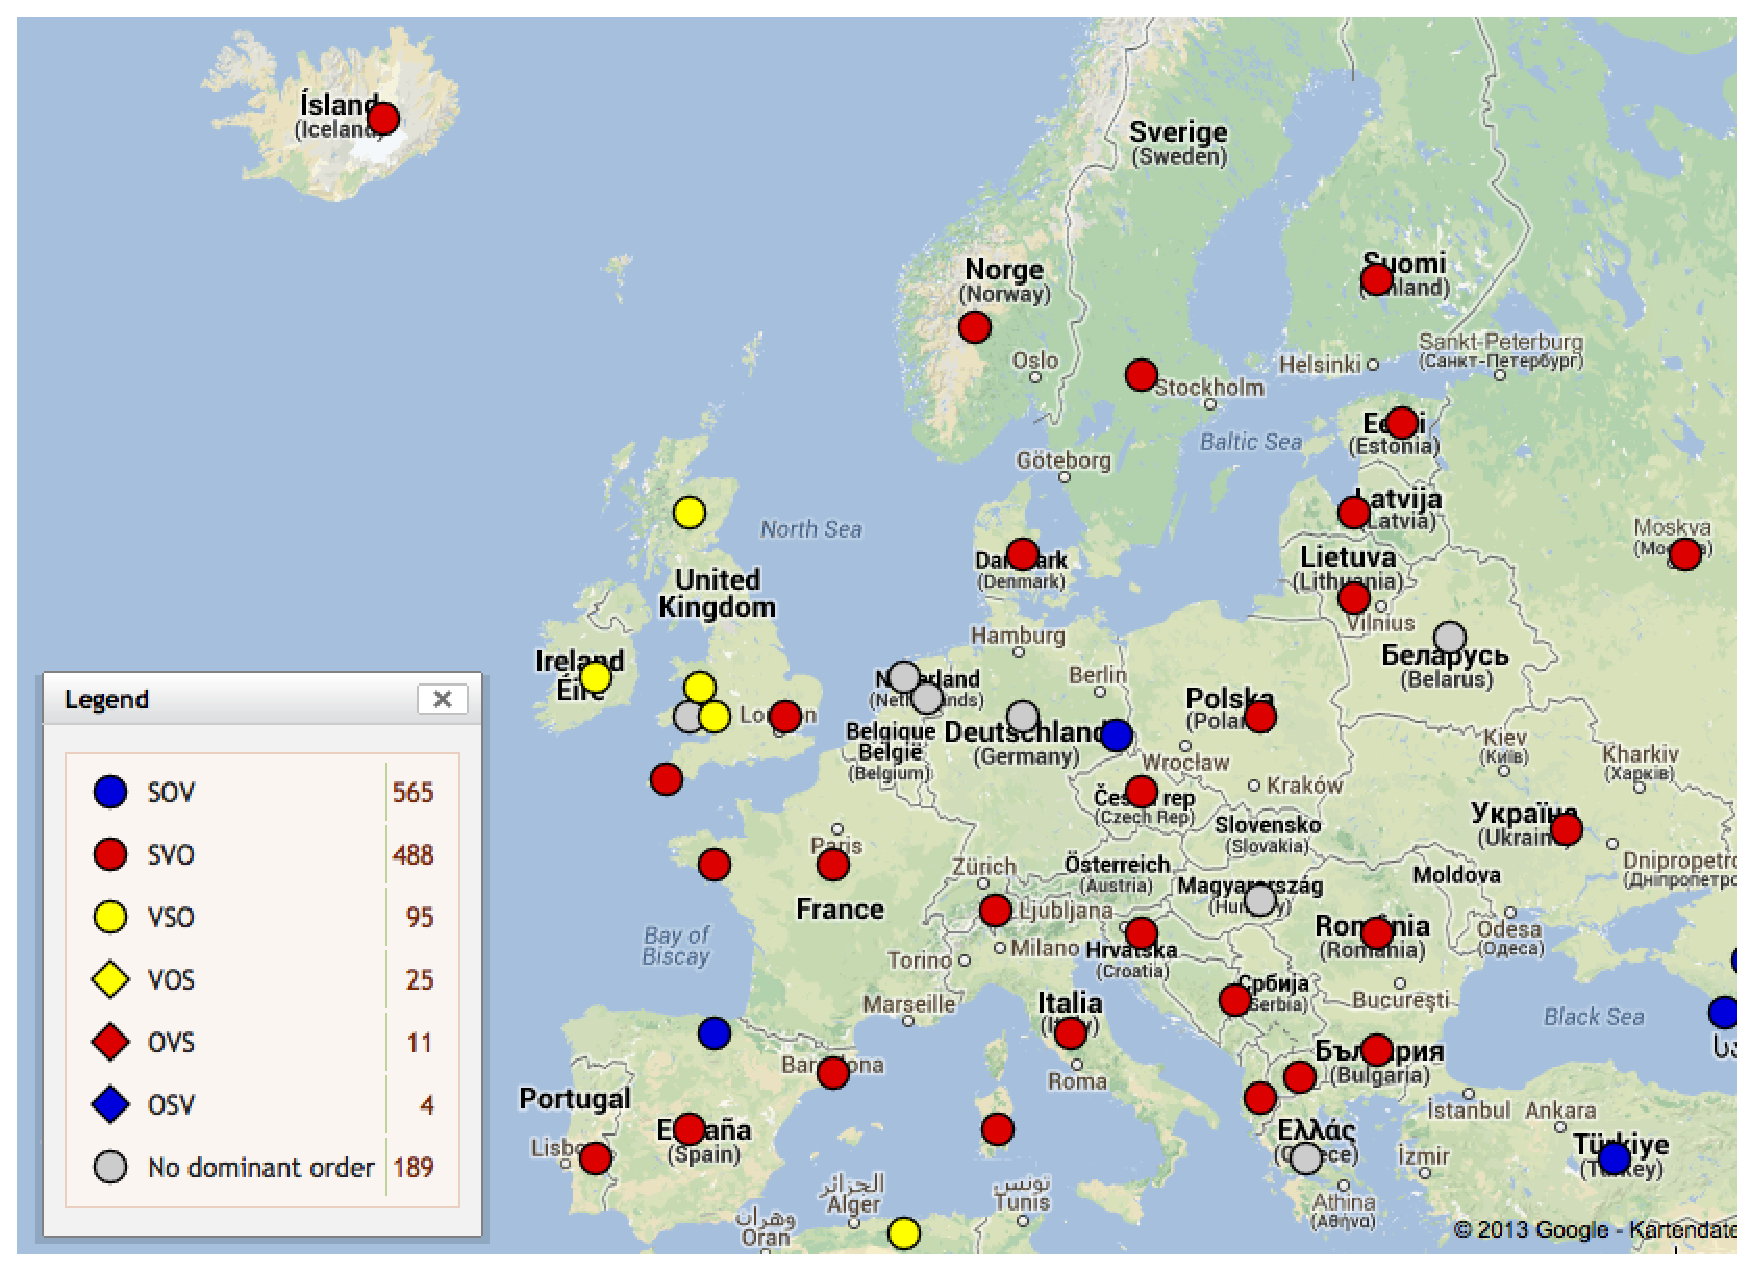
\includegraphics[width=.898\textwidth]{Pictures/WALS-SOV-Europa}
\caption{\label{fig-sov-wals-europe}Dominant orders of subject, object, and verb in Europe}
\end{figure}
According to the WALS the languages Icelandic, Norwegian, Swedish, Danish, and English are SVO
languages. Dutch, German, and Frisian, however, are marked in gray, that is, these languages are
marked to have no dominant order.\footnote{
  \citet[\page 87]{Greenberg63a-u} listed German and Dutch among the SVO languages.%
} According to Figure~\vref{fig-sov-wals-europe-two} these languages
have two dominant orders, namely SOV and SVO.
\begin{figure}
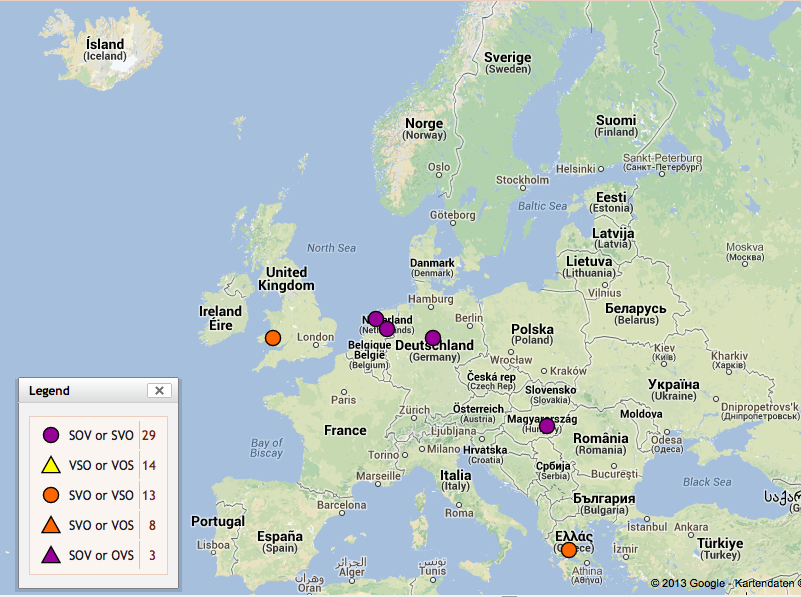
\includegraphics[width=.898\textwidth]{Pictures/WALS-SOV-Europa-no-dominant}
\caption{\label{fig-sov-wals-europe-two}%Dryer: Feature 81b: 
Two dominant orders of subject, object, and verb \citep[Section~3]{Dryer2013c}}
\end{figure}
%% https://wals.info/chapter/81
%% A third subtype of language lacking a dominant order consists of languages in which different word orders occur but the choice is syntactically determined. For example, in German and Dutch, the dominant order is SVO in main clauses lacking an auxiliary and SOV in subordinate clauses and clauses containing an auxiliary (see below for examples). Because this results in both orders being common, neither order is considered dominant here and these two languages are shown on the map as lacking a dominant word order. In general, if the word order varies according to whether there is an auxiliary verb, the language is shown on the map as lacking a dominant order. Another language whose word order depends both on whether there is an auxigermliary and whether the clause is a main clause is Dinka (Nilotic; Sudan): like German, the order is SVO in main clauses without an auxiliary, SAuxOV in main clauses with an auxiliary, but it is VSO in subordinate clauses without an auxiliary and AuxSOV in subordinate clauses with an auxiliary (Nebel 1948: 9, 25, 42, 75, 82).
The reason for this classification is that \citet[Section~1]{Dryer2013c} distinguishes between sentences in which the finite
verb is the main verb (\mex{1}a) and sentences in which the finite verb is an auxiliary as in (\mex{1}b):
\eal
\ex 
\gll Kim sieht den Fuchs.\\
     Kim sees the fox\\
\glt `Kim sees the fox.'
\ex
\gll Kim hat den Fuchs gesehen.\\
     Kim has the fox seen\\
\glt `Kim has seen the fox.'
\zl
According to Dryer the pattern for (\mex{0}a) is SVO and the one for (\mex{0}b) is SAuxOV, where Aux
stands for the auxiliary verb. Like
\citet{Greenberg63a-u}\footnote{%
  See \citew[\page 20--21]{HoehleTopo}.
}, Dryer counts the latter pattern as SOV order. The question is whether it is adequate to ignore auxiliaries
in the examination of constituent order. The auxiliary \emph{hat} `have' in (\mex{0}b) syntactically
behaves like the full verb \emph{scheint} `seems' in (\mex{1}):
\ea
\gll Kim scheint den Fuchs zu sehen.\\
     Kim seems   the fox  to see\\
\glt `Kim seems to see the fox.'
\z
So, here we would have an SVOV order, something that does not exist in the typology under discussion.
The languages in Figure~\ref{fig-sov-wals-europe-two} marked as not having a dominant order use the
verb position to mark the clause type: it is just the finite verb that is in first or second
position. Non-finite verbs are final: 
\ea
\gll Kim scheint den Fuchs gesehen zu haben.\\
     Kim seems   the fox  seen to have\\
\glt `Kim seems to have seen the fox.'
\z
In subordinate clauses we have both the finite verb and the non-finite verbs in final position while
the finite verb is in initial position\footnote{%
  I use the term initial position to refer to the position the finite verb has in V1 or V2 clauses. The
  analysis of V2 and V1 involves fronting of the finite verb. In V2 clauses, a constituent is fronted
  in addition.
} in questions and declarative main clauses.
A classification that is entirely based on counting patterns without taking auxiliary verbs and the
finiteness/non-finiteness distinction into account cannot tease these properties apart \citep[Section~3]{Hoehle83a}. In what follows we will have a look at clauses with
both finite and non-finite verbs. Such clauses reveal differences between OV and VO languages and I will argue that Afrikaans, Dutch,
German, and Frisian should be counted among the OV languages and that the other observable pattern
SVO is due to other properties of these languages, namely that they mark the clause type by verb
position and that they are verb"=second (V2) languages.\footnote{%
  The property of being a V2 language is independent of the SVO/SOV distinction. All Germanic
  languages except English are V2 languages. See Section~\ref{sec-phenomenon-v2} on V2.
}

When one builds more complex German sentences involving several verbs, the embedding verb is usually
realized to the right of the embedded verbs. 
%\itdopt{M: Are these notions defined somewhere?}
% Yes, in the text immediately following.
This is shown in (\mex{1}). (\mex{1}a) shows a simple
sentence with a finite verb. If we form the perfect as in (\mex{1}b), the perfect auxiliary has to
follow the participle. The auxiliary is the finite verb and it determines the form of the
participle. Hence the finite verb is the verb that embeds the participle. This is indicated by the
lower number of \emph{hat} in comparison to \emph{gesehen}. If we build an even more complex
sentence by adding another verb, this verb will be serialized to the right of the present verbs
(\mex{1}c).  The Danish example in (\mex{2}c), adapted from \citet[\page 146]{Oersnes2009b}, corresponds to the
German example in (\mex{1}c).

\eal
\ex
\gll dass sie ihn sieht$_1$\\
     that she him sees\\\jambox{(German)}
\glt `that she sees him'
\ex
\gll dass sie ihn gesehen$_2$ hat$_1$\\
     that she him seen        has\\
\glt `that she has seen him'
\ex
\gll dass sie ihn gesehen$_3$ haben$_2$ muss$_1$\\
     that she him seen        have     must\\
\glt `that she must have seen him'
\zl
\eal
\label{ex-Danish-embedding}
\ex
\gll at   hun ser$_1$ ham\\
     that she  sees    him\\\jambox{(Danish)}
\ex
\gll at   hun have$_1$ set$_2$ ham\\
     that she  has      seen    him\\
\ex
\gll at   hun må$_1$ have$_2$ set$_3$ ham\\
     that she  must   have     seen   him\\
\zl
%
As the examples in (\mex{0}) show, the verbs are added in front of the verbs they embed in
Danish. This is also the case for English as is evident from the glosses. In Danish and English the
verbs precede the object (\emph{ham}/\emph{him}) and in German they follow it (\emph{ihn}). 

\citet[Section~15.2]{Haider2020a} pointed out two further differences between the Germanic VO and OV languages:
particles precede verbs in OV languages and the same is true for resultative secondary
predicates. In VO languages particles and result predicates follow the verb. This is demonstrated by
the following two example sets:
\eal
\ex Kim will look up the information.
\ex 
\gll Kim wird die Information nachschlagen.\\
     Kim will the information \textsc{part}.beat\\\jambox{(German)}
\glt `Kim will look up the information.'
\zl
\eal
\ex Kim will fish the pond empty.
\ex 
\gll Kim wird den Teich leer fischen.\\
     Kim will the pond  empty fish\\\jambox{(German)}
\glt `Kim will fish the pond empty.'
\zl
(\mex{-1}a) shows that \emph{look} precedes the particle \emph{up}, while the verb \emph{schlagen}
`beat' has to follow the particle \emph{nach} in German. Similarly, the secondary resultative
predicate \emph{empty} follows the verb in (\mex{0}a), but \emph{leer} precedes the verb in
(\mex{0}b). Note that I used a future auxiliary in the examples in order to avoid side effects that
are due to the verb"=second property of German: in declarative main clauses the finite verb always
precedes particles and resultative predicates but this is due to the clause type (see Section~\ref{sec-phenomenon-v2}).

I will return to the SVO vs.\ SOV order in Chapter~\ref{chap-verb-position} and provide more
evidence that was used in the literature to argue for the OV status of languages like German and Dutch.
%\itdopt{M: descriptive OV status is compatible with comparative VO/OV classification.}

While the Germanic languages can be split nicely into SOV languages with scrambling (see
Section~\ref{sec-phenomenon-scrambling} below) and SVO languages without scrambling, there is one
exception: \ili{Yiddish}. The following data from \citet[\page 402]{Diesing97a} shows that Yiddish
can have the order usually observed in SVO languages (\mex{1}a) and the orders observed in SOV
languages with scrambling (\mex{1}b, c). But it can also have the orders in (\mex{1}d) and
(\mex{1}e), in which the verb is in the middle and either the direct object or the indirect object
precedes the verb.

\eal
\label{ex-yiddish-vo-ov}
\ex
\gll Maks hot nit gegebn Rifken dos bukh.\\
     Max  has not given  Rifken the book\\\yiddish
\glt `Max has not given Rifken the book.' 
\ex 
\gll Maks hot Rifken dos bukh nit gegebn.\\
     Max  has Rifken the book not given\\
\glt `Max has not given Rifken the book.'
\ex
\gll Maks hot dos bukh Rifken nit gegebn.\\
     Max  has the book Rifken not given\\
\glt `Max has not given Rifken the book.'
\ex
\gll Maks hot Rifken nit gegebn dos bukh.\\
     Max  has Rifken not given  the book\\
\glt `Max has not given Rifken the book.'
\ex
\glt Max hat dos bukh nit gegebn Rifken.\\
     Max has the book not given  Rifken.\\
\glt `Max has not given Rifken the book.'
\zl
Based on comparison with other Germanic languages, Yiddish was claimed to be a VO language
\parencites[\page 113]{dBMvW86a}[\page 388]{Diesing97a}{Sadock98a-u} or an OV
language \parencites{Hall79a-u}[\iaddpages]{Vikner2001a-u}. Some researchers argued that it is
neither but a third type of language, one with mixed VO/OV status \parencites{Santorini93a}[\page 12]{Schallert2007a}[\page 161]{Haider2010a}{Haider2020a}.

\citet[Section~2.5]{Schallert2007a} points out that many Germanic languages from earlier stages did not have a
fixed VO or OV order and assigns them together with Yiddish to this third class of languages with a
rather free verb position. His classification is given in Table~\ref{table-VO-OV}.
 
\begin{table}
\begin{tabular}{llll}\lsptoprule
               & OV-Sprachen        & VO-Sprachen        & OV/VO-Sprachen\\\midrule
North Germanic &                    & Islandic, Faroese, & Old Nordic \\
               &                    & Norwegian, Danish, & (Old Islandic)\\
               &                    & Swedish            &\\
West Germanic  & German, Dutch,     & English            & Jiddish, Old High \\
               & Afrikaans, Frisian &                    & German, Old English\\
\lspbottomrule
\end{tabular}
\caption{Constituent order typology of the Germanic languages according to \citet[\page 13]{Schallert2007a}}\label{table-VO-OV}
\end{table}


\section{V2}
\label{sec-phenomenon-v2}

The Germanic languages, with the exception of English, are so-called \emph{verb"=second languages} (V2
languages). The V2
property can be illustrated with the following German sentences. (\mex{1}) shows declarative main
clauses in which one of the constituents is fronted. (\mex{2}) shows parallel interrogative clauses.

\eal
\ex 
\gll Das Kind  gibt dem Eichhörnchen jetzt eine Nuss.\\
     the child gives the squirrel now a nut\\\jambox{(German)}
\glt `The child gives the squirrel a nut now.'
\ex 
\gll Dem Eichhörnchen gibt das Kind jetzt eine Nuss.\\
     the squirrel gives the child now a nut\\
\ex 
\gll Eine Nuss gibt das Kind dem Eichhörnchen jetzt.\\
     a nut gives the child the squirrel now\\
\ex 
\gll Jetzt gibt das Kind dem Eichhörnchen eine Nuss.\\
     now gives the child the squirrel a nut\\
\zl
\eal
\ex 
\gll Wer gibt dem Eichhörnchen jetzt eine Nuss?\\  
     who gives the squirrel now a nut\\\jambox{(German)}
\glt `Who gives the squirrel a nut now?'
\ex 
\gll Wem gibt das Kind jetzt eine Nuss?\\
     who gives the child now a nut\\
\glt `Who does the child give a nut to now?'
\ex 
\gll Was gibt das Kind dem Eichhörnchen jetzt?\\
     what gives the child the squirrel now\\
\glt `What does the child give the squirrel now?'
\ex 
\gll Wann gibt das Kind dem Eichhörnchen eine Nuss?\\
     when gives the child the squirrel a nut\\
\glt `When does the child give the squirrel a nut?'
\zl
The finite verb is in second position in all the sentences in (\mex{-1}) and (\mex{0}).


English, in contrast, does not allow orders in which the object appears immediately before the
finite verb.

\eal
\ex[*]{ 
This squirrel give I a nut now.
}
\ex[*]{
This nut give I a squirrel now.
}
\ex[*]{
Tomorrow give I the squirrel a nut.
}
\zl 
Adverbials and objects can be fronted but then they have to appear before the clause consisting of
subject and verb and possibly other constituents.
\eal
\ex This nut, I give the squirrel now. 
\ex Now, I give the squirrel a nut.
\zl

Note also that fronting of objects is restricted to the secondary object for verbs with two objects
for some speakers \citep[\page 258]{Hudson92a-u}.\footnote{
  I use the terms \emph{primary object}\is{object!primary} and \emph{secondary object}\is{object!secondary} in order to avoid confusion that is sometimes
  caused by the terms \emph{direct}\is{object!direct} and \emph{indirect object}\is{object!indirect}. The primary object is the first object in English
  and the dative object of ditransitive verbs governing the dative in German. The secondary object
  is the second object in English and the accusative in German ditransitive constructions. The order
  dative before accusative is also the unmarked order\is{order!unmarked} for arguments of most ditransitive verbs
  \citep{Hoehle82a}. For exceptions see \citew{Cook2006a-u}.
% Icelandic dat primary, acc secondary
% \itdopt{M: This is very confusing because the criterion is basically semantic (recipient vs. theme)
%   whereas primary seems to suggest syntactic criteria. It's the same confusion as with
%   direct/indirect.\\
% Stefan: Yes, we are doing syntax.}
} So, while fronting of the secondary object in
(\mex{1}b) is permitted by all speakers, some speakers find extractions like the extraction of the
primary object in (\mex{1}c) unacceptable or marked.
\vspace{-\baselineskip}
\eal
\judgewidth{\%}
\ex[]{
We give children sweets.
}
\ex[]{
These sweets, we give children \_.
}
\ex[\%]{
These children, we give \_ sweets.
}
\zl
This is not the case in V2 languages: they are rather liberal as far as fronting
is concerned. Basically all constituents can be fronted, exceptions being reflexive
pronouns that are selected by inherently reflexive verbs (\mex{1}), expletive objects (\mex{2}), and certain modal
particles (\mex{3}). See also \citew[\page 159]{Hoberg81a} on inherently reflexive verbs and modal particles.
\eal
\ex[]{
\gll Maria erholt sich.\\
     Maria recovers \REFL\\\german
\glt `Maria recovers.'
}
\ex[*]{
\gll Sich erholt Maria.\\
     \REFL{} recovers Maria\\
}
\zl
\eal
\ex[]{
\gll Er bringt es bis zum Professor.\\
     he brings \expl{} until to.the professor\\\german
\glt `He makes it to professor.'
}
\ex[\#]{
\gll Es bringt er bis zum Professor.\\
     \expl{} brings he until to.the professor\\
} 
\zl
\eal
\ex[]{
\gll Er geht halt nicht.\\
     he goes \textsc{particle} not\\\german
\glt `He simply does not go.'
}
\ex[*]{
\gll Halt geht er nicht.\\
     \textsc{particle} goes he not\\
}
\zl

The element in front of the finite verb is not necessarily a clause mate of the finite verb. In
fact, it can belong to a deeply embedded head as is demonstrated by the following example from
German:
\ea
\gll [Über dieses Thema]$_i$ habe ich sie gebeten, [[einen Vortrag \_$_i$~] zu halten]?\footnotemark\\
     \spacebr{}about this topic  have I her asked \hphantom{[[}a talk {} to hold\\\german
\footnotetext{
Adapted from \citew[\page 21]{HN89b}.
}
\glt `I asked her to give a talk about this topic.'
\z
The PP \emph{über dieses Thema} depends on \emph{Vortrag} `talk', which is part of the VP headed by
\emph{zu halten} `to hold', which is in turn embedded under \emph{gebeten} `asked'. Sentences like
(\mex{0}) show that V2 frontings cannot be analyzed as a simple reordering of the arguments of a
verb. While such an approach would work for the examples in (\mex{1}), it would not extend to other
cases in which the fronted element does not depend on the highest verb in the clause.
\ea
\gll Den Text kennt er.\\
     the.\ACC{} text knows he\\
\glt `He knows the text.'
\z

The following examples from Danish (SVO) show that the property of being a V2
language is independent of the VO/OV property:
\eal
\ex 
\gll Gert har læst bogen.\\
     Gert has read book.\textsc{def}\\\danish
\ex
\gll Bogen har Gert læst.\\
     book.\textsc{def} has Gert read\\
\zl
The example in (\mex{0}a) shows that the object follows the verbs and (\mex{0}b) shows that the
object \emph{bogen} `the book' can appear in sentence initial position in front of the finite verb
\emph{har} `have'.

The V2 order is used in declarative main clauses throughout the Germanic languages (without
English). Some Germanic languages do not use V2 order in embedded clauses. For a discussion of
embedded interrogatives see Section~\ref{sec-embeeded-clauses}.

While English does not allow for the order object"=verb"=subject, which is possible in the other Germanic
languages due to V2 fronting, it allows for the fronting of the object in questions resulting in
structures that are parallel to what we know from the other Germanic languages:
\eal
\ex Which book did Sandy read?
\ex Which book did Sandy give to Kim?
\ex To whom did Sandy give the book?
\zl
English used to be a V2 language but lost this property. The V2 in questions is a residue of earlier
stages of the language, which is why English is called a \emph{residual V2 language}\is{V2
  language!residual} \citep[\page 375]{Rizzi1990a-u}. 

V2 and verb fronting in general is a way to mark clause types in all Germanic languages. V2 sentence
can be declarative clauses in all Germanic languages except English and they can be questions in all
Germanic languages including English. In addition V2 sentences may be imperatives, as (\mex{1}) shows.
\ea
\gll Jetzt gib ihr das Buch!\\
     now give her the book\\\german
\glt `Give her the book now!'
\z
Sentences with the finite verb in first position (V1) can be yes/no questions or imperatives:
\eal
\ex
\gll Gibt er ihr das Buch?\\
     gives he her the book\\\german
\glt `Does he give her the book?'
\ex 
\gll Gib ihr das Buch!\\
     give her the book\\
\zl
Of course the order of elements is not the only cue as far as the clause type is
concerned. Intonation and morphological marking of imperative forms plays a role as well.

The property of being a V2 language is exceedingly rare among the world's languages \citep[\page
  343]{Holmberg2015a}. Apart from the Germanic languages with the exception of 
Modern English \citep{HP86a-ed}, there are only \ili{Estonian} (Finno-Ugric, \citealp[\page 343]{Holmberg2015a}), \ili{Sorbian} \citep[entry~79]{Plank2003b-ed} (a Slavic language), the
Celtic languages \ili{Breton} \citep{BK2000a-u}, \ili{Cornish} \citep*[\page 287]{BTW2007a-u}, and Middle \ili{Welsh} \citep{Willis1998a-u}, \ili{Old
  French} \parencites[Section~1.3]{Adams1987a-u}[Section~2.1.2]{Roberts93a-u}[Chapter~2]{Vance97a-u}, \ili{Old Spanish}
% Plank2003b-ed: and some other early Romance languages
%\citep{Fontana93a,Fontana97a}, 
\citep[Section~3.3.2]{Fontana97a-u}, 
\ili{Rhaeto"=Romance} \citep{Poletto2002a-u,Anderson2006a-u}, Kashmiri
\citep[Chapter~4]{Bhatt99a-u}, two dialects of \ili{Himachali}, which also belongs to Indo"=Aryan
and is spoken in regions adjacent to Kashmiri \citep{Hendriksen90a}, the Austronesian
languages \ili{Taiof} and \ili{Sisiqa} \citep[\page 495]{Ross2004a-u} and the Brazilian native
language \ili{Karitiana} from the language family Tupí \citep{Storto2003a-u}.
% This is mentioned in Bayer2010, but maybe it is like the australian languages.
% and the
%Uto-Aztekian language \ili{Tohono O'odham}, which is spoken in the southwest of the US and in northern Mexico.

% Estnisch 


\section{Scrambling}
\label{sec-phenomenon-scrambling}

While the constituent order in languages like English is rather fixed, languages like Dutch and
German allow a rather free permutation of arguments. In order not to contaminate the effects by
reorderings that are due to the V2 property, I use verb last sentences to illustrate the
phenomenon in German. Example (\mex{1}) shows the only possible order for subject and objects of a simple
ditransitive sentence in English without extraction:


\ea
because the child gives the squirrel the nut \jambox{(English)}
\z
If speakers want to realize the secondary object \emph{the nut} before the primary object \emph{the
  squirrel}, they have to use a prepositional object. This type of reordering is called
\emph{dative-shift} and an example is provided in (\mex{1}):
\ea
because the child gives the nut to the squirrel \jambox{(English)}
\z
In contrast to this we have the German examples in (\mex{1}). These examples show that the noun
phrases can be freely permuted:
\eal
\ex 
\gll {}[weil]          das Kind dem Eichhörnchen die Nuss gibt\\
     \spacebr{}because the child the squirrel the nut gives\\\jambox{(German)}
\ex 
\gll {}[weil]          das Kind die Nuss dem Eichhörnchen  gibt\\
     \spacebr{}because the child  the nut the squirrel gives\\
\ex 
\gll {}[weil]          die Nuss das Kind dem Eichhörnchen  gibt\\
     \spacebr{}because the nut the child  the squirrel gives\\
\ex 
\gll {}[weil]          die Nuss dem Eichhörnchen  das Kind gibt\\
     \spacebr{}because the nut the squirrel the child  gives\\
\ex 
\gll {}[weil]          dem Eichhörnchen  das Kind die Nuss gibt\\
     \spacebr{}because the squirrel the child  the nut gives\\
\ex 
\gll {}[weil]          dem Eichhörnchen  die Nuss das Kind gibt\\
     \spacebr{}because the squirrel the nut the child  gives\\
\zl
Not all of these orders can be used in all contexts. Some of the examples require a special,
contrastive intonation. The orders can be sorted with respect to the number of contexts in which
they can be used. \citet{Hoehle82a} suggests calling the order that can be used in most contexts the
normal or unmarked order\is{order!unmarked}.

The OV languages share a lot of properties, so one would expect that Dutch allows for scrambling as
well. However, NPs cannot be scrambled:
\ea[*]{
\longexampleandlanguage{
\gll Toen hebben de  autoriteiten het kind de moeder  teruggegeven\\
     then have   the authorities  the child the mother back.given\\}{Dutch}
\glt Intended: `The authorities gave back the child to the mother.'
}
\z
The reason for this is that NPs are not case marked in Dutch. It would be very difficult for hearers
and readers to find out who did what to whom. This is parallel to examples with caseless NPs in
German. As noted by \citet[\page 45]{Wegener85b}, (\mex{1}) is not ambiguous:
\ea
\gll Sie mischt Wein Wasser bei.\\
     she mixes  wine water  at\\\german
\glt `She mixes wine with water.'
\z
It means that there is wine and water is added to it. This corresponds to the order dat < acc.
The situation is different with determiners:
\eal
\ex 
\gll Sie mischt dem Wein das Wasser bei.\\
     she mixes  the.\DAT{} wine the.\ACC{} water at\\\german
\glt `She mixes wine with water.'
\ex Sie mischt das        Wasser dem        Wein bei.\\
    she mixes  the.\ACC{} water  the.\DAT{} wine at\\
\glt `She mixes wine with water.'
\zl
With determiners, we get the reading in (\mex{-1}) independent of the order of the noun phrases. If
we change the order of determinerless NPs in (\mex{-1}), we get a different reading:
\ea
\gll Sie mischt Wasser Wein bei.\\
     she mixes  water wine  at\\\german
\glt `She mixes water with wine.'
\z
So, without any clues from case marking, one has dat < acc order, with case marking, both orders are possible.

Returning to Dutch, the examples in (\mex{1}) show that scrambling is indeed possible, if the arguments can be
identified \parencites[\page 989]{GHdRvdT1984a-ed}[\page 14]{Haider2010a}:
\eal
\ex
\longexampleandlanguage{
\gll Toen hebben de autoriteiten het kind  aan de  moeder teruggegeven.\\
     then have   the authorities the child to  the mother back.given\\}{Dutch}
\ex 
\gll Toen hebben de  autoriteiten aan de moeder  het kind  teruggegeven\\
     then have   the authorities  to  the mother the child back.given\\
\zl
(\mex{0}) contains examples with NP and PP object. Since the PP is clearly identifiable, the two
arguments can appear in any order. Hence, it seems to be justified to assume that the OV languages (German,
Dutch, Afrikaans, Frisian) allow for scrambling with restrictions forbidding scrambling of elements that
are not identifiable.


\section{The position of adverbials}
\label{sec-phenomena-position-of-adverbials}

In languages like German and Dutch, the position of adverbials is rather free: the adverb \emph{gestern}
`yesterday' can appear anywhere between the arguments and the verb:
\eal
\ex
\longexampleandlanguage{
\gll weil das Kind dem Eichhörnchen die Nuss \emph{gestern} gab\\ 
     because the child the squirrel the nut yesterday gave\\}{German}
\glt `because the child gave the squirrel the nut yesterday'
\ex 
\gll weil das Kind dem Eichhörnchen \emph{gestern} die Nuss gab\\
     because the child the squirrel yesterday the nut gave\\
\ex 
\gll weil das Kind \emph{gestern} dem Eichhörnchen die Nuss gab\\
     because the child yesterday the squirrel the nut gave\\
\ex 
\gll weil \emph{gestern} das Kind dem Eichhörnchen die Nuss gab\\
     because yesterday the child the squirrel the nut gave\\
\zl
Dutch has free order of adverbials as well \parencites[\page
4]{Koster99a-u}[Section~6]{Bouma2003a-u}. (\mex{1}) shows the Dutch examples corresponding to (\mex{0}):
% Bouma2003a:6
% \eal
% \ex
% \gll dat  Kim regelmatig haar moeder bezoekt\\
%      that Kim regularly  her  mother visits\\\dutch
% \glt `that Kim visit her mother regularly'
% \ex
% \gll dat  Kim haar moeder regelmatig bezoekt\\
%      that Kim her  mother regularly  visits\\
% \glt `that Kim visit her mother regularly'
% \zl
\eal
\ex
\gll omdat het kind de eekhoorn de noot \emph{gisteren} gaf\\ 
     because the child the squirrel the nut yesterday gave\\\dutch
\glt `because the child gave the squirrel the nut yesterday'
\ex 
\gll omdat het kind de eekhoorn \emph{gisteren} de noot gaf\\
     because the child the squirrel yesterday the nut gave\\
\ex 
\gll omdat het kind \emph{gisteren} de eekhoorn de noot gaf\\
     because the child yesterday the squirrel the nut gave\\
\ex 
\gll omdat \emph{gisteren} het kind de eekhoorn de noot gaf\\
     because yesterday the child the squirrel the nut gave\\
\zl



In contrast, the position of the adverbials is rather restricted in SVO languages like Danish and
English. The adverbials usually are placed before or after the VP; that is, verb and objects form one
unit and adverbials attach to the left or to the right of this unit. (\mex{1}) provides an example:
\eal
\ex[]{
because the child {often} [gave the squirrel the nut] \jambox{(English)}
}
\ex[]{
because the child [gave the squirrel the nut] {often}
}
\ex[*]{
because the child [gave often the squirrel the nut]
}
\ex[*]{
because the child [gave the squirrel often the nut]
}
\zl
It is assumed that verb and objects form a structural unit, a verb phrase (VP). Adverbials may
attach to this VP forming a larger VP, which is than combined with the subject to form a complete sentence.

The following example, which is due to \citet[§ 8.20, 495]{QGLS85a-u}, shows that even in very
complex combinations of several verbs adverbs may be placed at the left periphery of a VP:
\ea
It [certainly [\sub{VP} may [possibly [\sub{VP} have [indeed [\sub{VP} been\\ {}[badly [\sub{VP} formulated]]]]]]]].
\z
This is different from the OV languages where verbs form a verbal complex which usually cannot be
interrupted by adverbs.
\eal
\ex[]{
\gll dass das Kind dem Eichhörnchen die Nuss morgen geben dürfen muss\\
     that the child  the squirrel the nut tomorrow give may must\\
\glt `that it must be possible that it is allowed that the child gives the squirrel the nut tomorrow'
}
\ex[*]{
\gll dass das Kind dem Eichhörnchen die Nuss geben morgen dürfen muss\\
     that the child  the squirrel the nut give tomorrow may must\\
}
\ex[*]{
\gll dass das Kind dem Eichhörnchen die Nuss geben dürfen morgen muss\\
     that the child  the squirrel the nut give  may tomorrow must\\
}
\zl

\section{Embedded clauses}
\label{sec-embeeded-clauses}

This section deals with embedded clauses that are introduced by a complementizer and with
embedded interrogative clauses. The Germanic languages vary with respect to the verb placement in
these subordinate clauses and with respect to the question whether the embedded clauses are V2 or not.

\subsection{Embedded clauses introduced by a complementizer}

As was already mentioned Afrikaans, Dutch, German are SOV languages and this is shown in embedded
clauses that are introduced by a complementizer. (\mex{1}) is an example:

\ea
\gll Ich weiß, dass Aicke das Buch heute gelesen hat.\\
     I know that Aicke the book today read has\\
\glt `I know that Aicke read the book today.'
\z


%% Stellung der anderen Konstituenten ist frei:
%% \eal
%% \ex Ich weiß, dass das Buch Max heute gelesen hat.
%% \ex Ich weiß, dass das Buch heute Max gelesen hat.
%% \zl

English, being an SVO non-V2 language allows for SVO order only.
\ea[]{
I  know that Kim has read the book yesterday. \jambox{(English)}
}
\z

Interestingly, Danish, also an SVO language, allows both SVO order (\mex{1}) and V2 order (\mex{2}) in clauses
preceded by a complementizer:
\ea[]{
\label{ex-at-max-ikke-har}
\gll Jeg  ved, at   Gert ikke  har læst   bogen          {i dag}.\\
     I know that Gert not has read book.\textsc{def} today\\\jambox{(Danish)}
\glt `I know that Gert did not read the book today.'
}
\z
%(Negation hilft, Verbstellung zu bestimmen)

\eal
\ex[]{
\gll Jeg  ved, at   {i dag} har Gert ikke læst bogen.\\
     I    know that today   has Gert not read book.\textsc{def}\\\jambox{(Danish)}
}
\ex[]{
\gll Jeg  ved, at   bogen          har Gert ikke  læst {i dag}.\\
     I know that book.\textsc{def} has Gert not read today\\
}
\zl
The example in (\ref{ex-at-max-ikke-har}) includes the negation in order to show that we indeed deal
with the SVO order here. Without the negation it is not clear whether non-V2 clauses are allowed in
clauses that are introduced by a complementizer since (\mex{1}a) has the finite verb in second
position. With the negation present, it is clear that we have a V2 clause if the negation follows
the finite verb and that we do not have a V2 clause if the finite verb follows the negation as in
(\mex{-1}) and hence is in third position.
\eal
\settowidth\jamwidth{(V2 or SVO)}
\ex 
\gll at Gert har læst bogen\\
     that Gert has read book.\textsc{def}\\\jambox{(V2 or SVO)}
\ex 
\gll at Gert har ikke læst bogen\\
     that Gert has not read book.\textsc{def}\\\jambox{(V2)}
\zl 
For complementizerless sentences the V2 order is the only one that is possible:
\eal
\settowidth\jamwidth{(V2 or SVO)}
\ex[]{ 
\gll Gert har ikke læst bogen\\
     Gert has not read book.\textsc{def}\\\jambox{(V2)}
}
\ex[*]{ 
\gll Gert ikke har læst bogen\\
     Gert not  has read book.\textsc{def}\\\jambox{(SVO)}
}
\zl 


Yiddish and Icelandic are SVO languages as well. The clauses that are combined with a
complementizer are V2:
\eal
\ex
\gll Ikh meyn  az   haynt hot Max geleyent dos bukh.\footnotemark\\
     I think that today has Max read the book\\\yiddish
\footnotetext{\citew[\page 58]{Diesing90a}}
\glt `I think that Max read the book today.'

\ex% check!
\gll Ikh meyn  az   dos bukh hot Max geleyent.\\
     I think that the book has Max read\\

\zl
\ea 
\gll Engum         datt í hug,  að   vert  væri að reyna til     að kynnast honum.\footnotemark\\
     no.one.\DAT{} fell to mind that worth was  to try   \PREP{} to know    him\\\icelandic
\footnotetext{\citew[\page 75]{Maling90a-u}}
\glt `It didn't occur to anyone that it was worth trying to get to know him.'
\z

\subsection{Interrogative clauses}


The OV languages form subordinated interrogative clauses by preposing a phrase containing an
interrogative pronoun\footnote{
Most interrogative pronouns start with \emph{w} in German and \emph{wh} in English. Phrases
containing an interrogative pronoun are called \emph{w}"=phrases or \emph{wh}"=phrases,
respectively. Interrogative clauses are sometimes called \emph{w}"=clauses or \emph{wh}"=clauses.
} from an
otherwise SOV clause. (\mex{1}) shows a German example:
\eal
\ex 
\gll Ich weiß, wer heute das Buch gelesen hat.\\
     I know    who today the book read has\\\jambox{(German)}
\glt `I know who read the book today.'
\ex 
\gll Ich weiß, was Aicke heute gelesen hat.\\
     I know    what Aicke today read has\\
\glt `I know what Aicke has read today.'
\zl
Since languages like German allow for scrambling, sentences like those in (\mex{0}) could just be due
to the permutation of arguments of a head. However, the generalization about these \emph{w}"=clauses
is that an arbitrary \emph{w}"=element can be fronted. (\mex{1}) gives an example from German that
involves a nonlocal dependency:
\ea
\gll Ich weiß nicht, [über welches Thema]$_i$ sie versprochen hat,~~~~~~~~ [[einen Vortrag \_$_i$] zu halten].\\
     I know not      \spacebr about which topic she promised has \hphantom{[[}a talk to  hold\\\jambox{(German)}
\glt `I do not know about which topic she promised to give a talk.'
\z
Here, the phrase \emph{über welches Thema} `about which topic' is an argument of \emph{Vortrag},
which is embedded in the VP containing \emph{zu halten} `to hold', which is in turn embedded under
\emph{versprochen hat} `promised has'. The generalization about interrogative clauses is that an
interrogative clause consists of a interrogative phrase (\emph{über welches Thema} `about which
topic') and a clause in which this interrogative phrase is missing somewhere (\emph{er versprochen
  hat, einen Vortrag zu halten} `he promised to give a talk').

In German the order of the other constituents is free as in assertive main clauses and embedded
clauses with a complementizer that were discussed earlier. 
\eal
\ex
\gll Ich weiß, was keiner diesem Eichhörnchen geben würde.\\
     I know    what nobody this squirrel give would\\\jambox{(German)}
\glt `I know what nobody would give this man.'
\ex 
\gll Ich weiß, was diesem Eichhörnchen keiner geben würde.\\
     I know what this squirrel nobody give would\\
\zl

In Danish and English the interrogative clauses consist of an interrogative phrase and an SVO clause
in which it is missing:
\eal
\ex 
\gll Gert har givet ham bogen.\\
     Gert has given him book.\textsc{def}\\\jambox{(Danish)}
\glt `Gert gave him the book.'
\ex
\gll Jeg ved, hvad$_i$ [Gert har givet ham \_$_i$].\\
     I know what \spacebr{}Gert has given him\\
\glt `I know what Gert gave him.'
\ex
\gll Jeg ved, hvem$_i$ [Gert har givet \_$_i$   bogen].\\
     I know who        \spacebr{}Gert has given {} book.\textsc{def}\\
\glt `I know who Gert has given the book.'
\zl
(\mex{0}a) shows the clause with SVO order and (\mex{0}b) is an example with the secondary object as
interrogative pronoun and (\mex{0}c) is an example with the primary object as interrogative
pronoun. The position that the respective objects have in non-interrogative clauses like (\mex{0}a)
is marked with \_$_i$.

Yiddish is special in that it has a V2 order in interrogative clauses as well \citep[Sections~4.1, 4.2]{Diesing90a}: interrogatives
consist of a interrogative phrase that is extracted from a V2 clause:

\ea
\gll Ir veyst efsher [avu            do    voynt Roznblat   der goldshmid]?\footnotemark\\
     you know maybe  \spacebr{}where there lives Roznblat the goldsmith\\
\glt `Do you perhaps know where Roznblat the goldsmith lives?' 
% The gollsing an translation differes in the original Rozenblatt
\footnotetext{
\citew[\page 65]{Diesing90a}. Quoted from Olsvanger, \emph{Royte Pomerantsn}, 1949.
}
\z

%% \eal 
%% \ex
%% \label{vosmaks}
%% \gll Ikh veys nit   vos$_i$ [Max hot gegesn \_$_i$].\footnotemark\\
%%      I know not     what \hphantom{[}Max has eaten\\
%% \footnotetext{\citew[\page 68]{Diesing90a}.}
%% \glt `I do not know what Max has eaten.'

%% \ex%check
%% \gll Ikh veys nit   [vos                    hot Max gegesn].\footnotemark\\
%%      ich weiß nicht \hphantom{[}was heute hat Max gegessen\\
%% \footnotetext{\citew[S.\,68]{Diesing90a}.}
%% \glt `Ich weiß nicht, was Max heute gegessen hat.'
%\zl
So the variation is \emph{w}-phrase + SOV, \emph{w}-phrase + SVO, and \emph{w}-phrase + V2.


\section{The use of expletives to mark the clause type}

The Germanic languages use constituent order to code the clause type: V2 main clauses can be
assertions or questions, depending on the content of the preverbal material and
intonation. Similarly embedded interrogative clauses consist of a \emph{w}"=phrase and an SVO, SOV,
or V2 clause. The fronting of a constituent in a V2 clause comes with certain information structural
effects: something is the topic or the focus of an utterance. For embedded sentences it is important
for some languages that the structure is transparent that is that we have the \emph{w} + SVO or
\emph{w} + V2 order. There are situations in which it is inappropriate to front an element and in
such situations the Germanic languages use expletives, that is, pronouns that do not contribute
semantically, to maintain a certain order.

German uses the expletive \emph{es} to fill the position in front of the finite verb, if no other
constituent is to be fronted.
\eal
\ex 
\gll Drei Reiter ritten zum Tor hinaus.\\
     three riders rode  to.the gate out\\\german
\glt `Three riders rode out of the gate.'
\ex 
\gll Es ritten drei Reiter zum Tor hinaus.\\
     \expl{} rode   three riders to.the gate out\\
\zl

Danish uses the expletive to make it clear that an extraction of a constituent took place
\citep[\page 169]{MOe2011a}:\footnote{
  Examples marked with DK are extracted from KorpusDK, a corpus of 56 Million words documenting
  contemporary Danish (\url{http://ordnet.dk/korpusdk}).
}
\eal
\ex[]{
\gll Politiet            ved   ikke,  hvem der           havde placeret bomben.\footnotemark\\
     police.\textsc{def} knows not    who  \textsc{expl} has placed bomb.\textsc{def}\\\danish
\footnotetext{DK}
\glt `The police does not know who placed the bomb.'
}
\ex[*]{
\gll Politiet ved ikke,  hvem havde placeret bomben.\\
     police.\textsc{def} knows not who has placed bomb.\textsc{def}\\
}
\zl
Without the expletive one would have a pattern like the one in (\mex{0}b). In (\mex{0}b) we have the
normal SVO order and it is not obvious to the hearer that the pattern consists of an extracted
element (the subject) and an SVO clause from which it is missing. This is more transparent if an
expletive is inserted into the subject position as in (\mex{0}a). (\mex{1}) shows this using the
analysis that will be suggested in Chapter~\ref{chap-expletives}: (\mex{1}a) shows the hypothetical
structure that would result if one assumed that the subject \emph{hvem} `who' is
extracted. So-called \emph{string-vacuous movement} would result: the subject is moved to a place
right next to it. In (\mex{1}b) on the other hand the subject position is taken by the expletive and
hence it is clear that the embedded sentence has a special structure. There is an overt marker for
the hearer or reader of the sentence marking it as an embedded interrogative clause.
\eal
\ex[*]{ 
\gll [hvem$_i$     [\trace$_i$ havde placeret bomben]]\\
     \spacebr{}who {}          has placed bomb.\textsc{def}\\\danish
}
\ex[]{
\gll [hvem$_i$     [der                    havde \trace$_i$ placeret bomben]]\\
     \spacebr{}who \spacebr{}\textsc{expl} has   {}         placed bomb.\textsc{def}\\
}
\zl

Similarly Yiddish uses an expletive in embedded interrogatives (\emph{w} + V2) if 
%the subject is extracted and 
there is no other element that is information structurally appropriate for the preverbal position.
%% \ea
%% \label{vosmaks}
%% \gll Ikh veys nit   [vos Max hot gegesn].\footnotemark\\
%%      ich weiß nicht \hphantom{[}was Max hat gegessen\\
%% \footnotetext{\citew[S.\,68]{Diesing90a}.}
%% \glt `Ich weiß nicht, was Max gegessen hat.'
%% \z
%% 
%% \item 
(\mex{1}) shows examples from \citet[\page 403--404]{Prince89a}:

\eal
\ex[]{
\gll ikh hob  zi  gefregt ver es         iz beser  far ir\\
     I   have her asked   who \textsc{expl} is better for her\\\yiddish
\glt `I have asked her who is better for her.'}
\ex[]{
\gll ikh hob  im  gefregt vemen es        kenen ale dayne khaverim\\
     I   have him asked   whom \textsc{expl} know  all your friends\\
\glt `I asked him whom all your friends know.'}
\zl
(\mex{0}a) is an example involving an interrogative pronoun that is the subject and (\mex{0}b) is an
example in which the preverbal position is not filled by an argument of \emph{kenen} `know' but by
an expletive. The subject \emph{ale dayne khaverim} `all your friends' stays behind and the object
\emph{vemen} `whom' is extracted since it is the interrogative pronoun.



\section{Verbal complexes in OV languages}


The OV languages have a verbal complex, or more general, a predicate complex, since adjectives take
part in complex formation as well. (\mex{1}) gives a German example by Haider (\citeyear[\page
  110]{Haider86c}; \citeyear[\page 128]{Haider90b}):
\ea
\gll weil es ihr jemand zu lesen versprochen hat\\
     because it.\ACC{} her.\DAT{} somebody.\NOM{} to read promised has\\\german
\glt `because somebody promised her to read it'
\z
The arguments of the respective verbs can be mixed with arguments of other verbs. In the example
above the \emph{es} `it' is not adjacent to its verb \emph{lesen} `to read', neither is \emph{ihm}
`him' adjacent to \emph{versprochen} `promised' nor \emph{jemand} to \emph{hat} `has'. In a more
``well-behaved'' ordering the object of \emph{zu lesen} `to read' is adjacent to the verb:
\ea
\gll weil    jemand   ihr das Buch zu lesen versprochen hat\\
     because somebody her the book to read  promised    has\\
\glt `because somebody promised her to read the book'
\z
The ordering in (\mex{0}) would allow for an analysis in which \emph{das Buch zu lesen} forms a VP
which is treated as an argument of \emph{versprochen} `promised'. However, this is not a viable
analysis for (\mex{-1}) if one assumes that phrases have to be continuous.

One explanation of orders like the one in (\mex{-1}) is that the verbs form a unit that behaves like a simplex verb. As with
the ditransitive verb \emph{geben} `to give' all permutations of the arguments of the verbs are
possible in principle. So \emph{zu lesen versprochen hat} forms a complex in both (\mex{-1}) and
(\mex{0}) and all permutations of the three arguments are permitted by the grammar.

VO languages like English and Danish do not allow permutations of arguments that belong to different
verbs. In VO languages governing verbs always embed VPs. The following example indicates the
structure:
\ea
because somebody [will [promise him [to read the book]]]
\z



\section{Obligatoriness of subjects, case of subjects, and passives}

SVO languages like English and Danish require a subject, while OV languages like German allow for
subjectless constructions.
\eal
\ex 
\gll Ihm graut vor der Prüfung.\\
     him.\DAT{} dreads before the exam\\\german
\glt `He dreads the exam.'
\ex 
\gll Heute wird nicht gearbeitet.\\
     today is   not worked\\
\glt `There is no working today.'
\zl
According to the tests that were used for languages like Icelandic (for instance the possibility to
omit a subject in infinitival constructions), the dative object \emph{ihm} `him' in (\mex{0}a) is
not a subject. There is no nominal argument at all in (\mex{0}b). As we will discuss in
Section~\ref{sec-icelandic-quirky-subj}, Icelandic has dative subjects \citep{ZMT85a}, which makes it the most
exciting language to study among the Germanic languages. We will see that a uniform analysis of case
assignment is possible \citep*{YMJ87}, although there is some variety in the inflectional systems of the Germanic languages.


As is shown in (\mex{0}b), German allows for so-called impersonal passives. Impersonal passives are
a special kind of passives in which no element gets promoted to subject. SVO languages like English,
Danish do not allow subjectless constructions. English therefore does not allow impersonal passives
at all as (\mex{1}b) shows:
\eal
\ex[]{
\label{ex-gearbeitet-wurde}
\gll weil noch gearbeitet wird\\
     because still worked is\\\german
\glt `because there is still working there'
}
\ex[*]{
because (it) was worked \english
}
\zl
Interestingly, Danish found a way to fulfill the subject requirement and at the same time have
impersonal passives: Danish simply inserts an expletive pronoun into the subject position:
\eal
\label{ex-bliver-arbejder}
\ex 
\gll fordi der bliver arbejdet\\
     because \textsc{expl} is worked\\\danish
\glt `because there is working there'
\ex
\gll fordi   der arbejdes\\
     because  \textsc{expl} work.\textsc{pass}\\
\glt `because there is working there'
\zl
German does not allow for an expletive subject:
\ea[*]{
\gll  weil es noch gearbeitet wird\\
      because it still worked is\\\german
\glt `because there is still working there' 
}
\z
It is possible to have an expletive pronoun in front of the finite verb as in (\mex{1}), but this is
a positional expletive whose purpose it is to mark the V2 sentence type. 
\ea
\gll  Es wird noch gearbeitet.\\
      \textsc{expl} is still worked\\\german
\glt `There is still working there.'
\z
The expletive is not an argument of any verb. The purely positional character of this expletive is shown by the fact that it does not
appear in verb last sentences like (\mex{-1}).

\section{Summary}

This chapter provided an overview of the phenomena that are covered in this book. Of course we will
look at everything in much more detail in the chapters to come. Let's start and get our hands dirty.


\questions{

\begin{itemize}
\item What is the characteristics of a V2 language?
\item If a language has many sentences with subject, verb, object order, do you know that the language
  is a V2 language?
\end{itemize}

}

\furtherreading{
The book \emph{Germanic languages} edited by \citet{KvdA94a-ed} provides a descriptive overview of
the Germanic languages.
}


%      <!-- Local IspellDict: en_US-w_accents -->
